\newpage
\section{Exercises: Frequency Response}

\begin{enumerate}

\item The impulse response of an LTI system is defined as:
\begin{equation}
    h(t) = \frac{42\sin(\omega_c t)}{\pi t}.
    \label{eq:ir_42rect}
\end{equation}
The input to the LTI system is a periodic signal with a fundamental period $T=1$:
\begin{equation}
    x(t) = \sum_{n=-\infty}^{\infty}\delta(t-n).
\end{equation}
When the signal $x(t)$ is fed into an LTI system, the output signal is given by a convolution of the input signal with the output signal:
\begin{equation}
    y(t) = \int_{-\infty}^{\infty} h(t-\tau)x(\tau) d\tau.
\end{equation}
\begin{enumerate}[a)]
\item Determine the Fourier transform $\hat{x}(\omega)$ of the input signal. Plot $\hat{x}(\omega)$ over the range of angular frequencies $-7\pi < \omega < 7\pi$. Hint: It might help if you start by expressing the signal $x(t)$ using a Fourier series representation first, and then apply Equation \ref{eq:fsftgen}.
\item Determine the frequency response $\mathcal{H}(\omega)$ of the LTI system. In other words, Fourier transform the impulse response signal given in Equation \ref{eq:ir_42rect}. It should be a fairly simple function. Make a plot of $|\mathcal{H}(\omega)|$ on the same graph as $\hat{x}(\omega)$ using $\omega_c = 5\pi$.
\item Use your plot in b) to determine $y(t)$, the output of the LTI system characterized using $h(t)$ when $\omega_c=5\pi$. Hint: use property that convolution in time domain is multiplication in frequency domain.
\item What values of $\omega_c$ will result in a non-zero constant output $y(t)=c$. What is the constant $c$?
\end{enumerate}

\item A running average filter is defined as:
  \begin{equation}
    y[n] = \frac{1}{M} \sum_{k=0}^{M-1} x[n-k].
    \label{eq:racausal}
  \end{equation}
  This filter only depends on the current and past values of the input, and can thus be implemented in a real-time system. Assume that $M$ is an odd number.
  \begin{enumerate}[a)]
  \item What is the impulse response $h_M[n]$ of the system described in Equation \ref{eq:racausal}?
  \item What is the frequency response $\mathcal{H}_M(\hat{\omega})$ of the system described in Equation \ref{eq:racausal}?
  \item What is the frequency response $\mathcal{H}_{\tau}(\hat{\omega})$ of a time-shift system $h_{\tau}[n]=\delta[n-\tau]$?
  \item I recommend that you do this task on a computer. Plot the squared magnitude response $|\mathcal{H}_M(\hat{\omega})|^2$ between $-\pi < \hat{\omega} < \pi$. Assume that $M=11$. Compare this with a plot of the squared magnitude response of the time-symmetric running average filter $|D_M(\hat{\omega})|^2$ of the same length. It is defined in Equation \ref{eq:dirikereq}. They should be the same. If you are not sure why, carry on with the next tasks.
  \item Show that the frequency response $\mathcal{H}_M(\hat{\omega})$
     be obtained by multiplying the frequency response of the time symmetric running average filter given in Equation
    \ref{eq:dirikereq} with the frequency response of the time shift system with a suitable value of $\tau$:
    \begin{equation}
      \mathcal{H}_M(\hat{\omega}) =
    D_{M}(\hat{\omega})\mathcal{H}_{\tau}(\hat{\omega})?
    \end{equation}
    Hint: Look at the derivation of $D_M(\hat{\omega})$.
    \item Explain why $|\mathcal{H}_M(\hat{\omega})|^2=|\mathcal{D}_M(\hat{\omega})|^2$. Hint: $|z|^2 = z z^*$.
  \end{enumerate}

\begin{marginfigure}
\begin{center}
        \begin{tikzpicture}
        \begin{axis}[width=6cm,height=6cm,ymin=-2.5,ymax=2.5,xmin=-4,xmax=4,
    xlabel={$n$}, ylabel={$h[n]$}, axis lines = center]
    
   \addplot+[ycomb] plot coordinates {(-3,0) (-2,0) (-1,1) (0,-2) (1,1) (2,0) (3,0) (3,0)};
        \end{axis}
        \end{tikzpicture}
\end{center}
\caption{The impulse response of a second order derivative estimator filter with $T_s=1$.}
\label{fig:exer_laplac}
\end{marginfigure}


\item It is possible to numerically estimate the second time
  derivative of a discretized signal using an FIR filter with the
  following filter coefficients:
  \begin{equation}h[n]= T_s^{-2}\delta[n+1] -2
    T_s^{-2}\delta[n] + T_s^{-2}\delta[n-1]
    \label{eq:fir_diff_filter}
    \end{equation}
  where $T_s$ is the sample spacing. This can be motivated by the following definition of a second time-derivative:
  \begin{equation}
    \frac{d^2x}{dt^2} = \lim_{T_s \rightarrow 0} \frac{x(t+T_s)-2x(t)+x(t-T_s)}{T_s^2}
  \end{equation}
  which is numerically evaluated with a finite difference $T_s$.

 If a signal of the form $x[n]=A e^{i\phi}e^{i\hat{\omega} n }$ is fed into the FIR filter described by an impulse response $h[n]$,
  the output signal will be of the form $y[n]=A' e^{i \phi'} e^{i \hat{\omega}n}$.
  Here $A,A'\in \mathbb{R}_{\ge 0}$ and $\hat{\omega},\phi,\phi' \in \mathbb{R}$.

  
  \begin{enumerate}[a)]
  \item Show that the frequency response of this filter is
    \begin{equation}
      \mathcal{H}(\hat{\omega}) = \frac{2}{T_s^{2}}[\cos(\hat{\omega})-1]
    \end{equation}
  \item Make a plot of the magnitude response $|\mathcal{H}(\hat{\omega})|$ between normalized angular frequencies $-\pi < \hat{\omega} < \pi$ (radians per sample).
  \item What is the phase response $\angle \mathcal{H}(\hat{\omega})$ of this system?
    
  \item Is this filter a high-pass or a low-pass filter? 
  \item What is $A'$ when $\hat{\omega}=0$?
  \item What is $A'$ and $\phi'$ when $\hat{\omega}=\pi/2$ and $\hat{\omega}=\pi$?
  \item Show that for continuous-time signals, the second
    time-derivative operation $\mathcal{T}\{x(t)\} =
    \frac{d^2}{dt^2}x(t)$ has a frequency response of the form
    $\mathcal{H}(\omega)=-\omega^2$.

  \item A plot of the continuous-time frequency response found in g) and the discrete-time frequency response found in a) is shown in Figure \ref{fig:ct_dt_laplacian}. The sample spacing is assumed to be $T_s=1$. With this sample spacing, both $\omega$ and $\hat{\omega}$ will have the same scale ($\omega = 1$ rad/s will correspond to $\hat{\omega}=1$ rad/sample). What does the plot tell you about how well the FIR filter in Equation \ref{eq:fir_diff_filter} approximates the second time derivative operation for continuous-time complex sinusoidal signals as a function of frequency?
\end{enumerate}


\begin{marginfigure}[-5cm]
\begin{center}
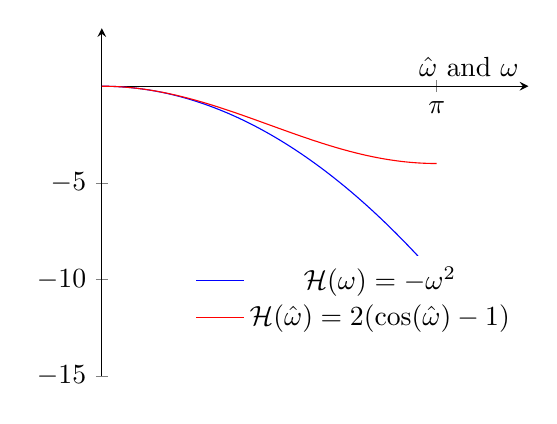
\begin{tikzpicture}
	\begin{axis}[width=7cm,
        height=6cm,
        domain=(0):(3.14),
        samples=200,
        xmin=0,
        xmax=4,
        ymin=-15.0,
        ymax=3,
    legend style={draw=none,at={(.99,.1)},anchor=south east},
        xlabel={$\hat{\omega}$ and $\omega$},
	    ylabel={},
        axis x line=center, 
    axis y line=middle,
    xtick={0,3.14},
    xticklabels={0,$\pi$}
%    legend pos=south east
    ]
          \addplot[blue] {-x*x};
          \addlegendentry{$\mathcal{H}(\omega)=-\omega^2$};
          \addplot[red] {2*(cos(deg(x))-1)};
          \addlegendentry{$\mathcal{H}(\hat{\omega})=2(\cos(\hat{\omega})-1)$};
    \end{axis}
\end{tikzpicture}
\end{center}
\caption{The frequency response of a continuous-time second time-derivative operation and a numerical estimator of the second time-derivative in discrete-time.}
\label{fig:ct_dt_laplacian}
\end{marginfigure}
\vspace{3cm}


\end{enumerate}
